\chapter{Introduction to statistics}
% TODO missing statistics concepts
% - http://sahilmohnani.wordpress.com/2013/06/02/absolute-mean-deviation/
% - http://sahilmohnani.wordpress.com/2013/06/03/a-multiple-linear-regression-wait-what-did-i-read-that-correctly

John Graunt as unusual and earned him a revered place in the history books is an eighty-five-page pamphlet published in 1662 and titled Natural and Political Observations Made Upon the Bills of Mortality.

In it, Graunt organized and analyzed the mortality rolls of London at that time, in an attempt to create a system to warn of the onset and spread of plague in the city. This work marked the beginning of modern statistics

The focus of Major Graunt’s booklet was the bills of mortality that had been collected by the London parishes since 1604. The Company of Parish Clerks published the weekly bills along with an annual bill that summarized the entire year.

Graunt often displayed considerable ingenuity in teasing important facts from lists of numbers. When rickets first began to appear as a cause of death, a natural question was whether this was a new disease or simply a new classification for an ailment that had long been in existence. By comparing the rate of increase of burials recorded as due to rickets with the rate of burials overall, Graunt concluded that rickets was in fact a new disease with an increasing mortality.

A figure of particular interest to the government was the number of men in London of fighting age (defined to be between sixteen and fifty-six). To determine this number, Graunt calculated age-related mortality rates. This marked the introduction of what rapidly became a hugely important concept: the life-expectancy table, the basis for the life insurance industry.

Graunt’s life-expectancy table leaves much to be desired in both accuracy and method. But it was the first attempt in human history at generating such data. Within a short time of the publication of his Observations, life-expectancy tables were used widely in medical statistics, demography, and actuarial science, as well as providing the foundation for a rapidly expanding (and still thriving) business of selling life annuities.

\section{Data visualization}
When studying data in order to make better decisions we often start by looking for patterns of behavior. The simplest form of pattern is the number of times a specific data value occurs also known as its frequency. For example when schools create learning plans for classes they analyze frequency of the class grades. Armed with this knowledge special measures can be taken, such as splitting the class into multiple groups to be thought separately.

For example, if four students receives an $F$ in mathematics, then the grade $F$ is said to have a frequency of $4$. The frequency of a data is often represented in a table by arranging data values in ascending order of magnitude with their corresponding frequencies. For example on a $A, B, C, D, F$ grading scale the grades $A, A, B, B, B, C, C, D, F$ produces the following frequency table
\begin{table}[H]
\centering
\begin{tabular}{|l|l|}
\hline
\textbf{Grade} & \textbf{Frequency} \\ \hline
A              & 2                  \\ \hline
B              & 3                  \\ \hline
C              & 2                  \\ \hline
D              & 1                  \\ \hline
F              & 1                  \\ \hline
\end{tabular}
\end{table}
the table above can be easily visualized in a frequency plot, where each dot represents a occurrence of the value below
\begin{figure}[H]
\centering
\begin{tikzpicture}
\begin{axis}[
    symbolic x coords={A,B,C,D,F},
    hide y axis,
    axis x line*=bottom,
    height=4cm,
    width=10cm
]
\addplot+[only marks] plot coordinates
	{(A,1) (A, 2) (B,1) (B,2) (B,3) (C,1) (C,2) (D,1) (F,1)};
\end{axis}
\end{tikzpicture}
\end{figure}
from this frequency plot we can easily deduce that the most common grade in the exam was $B$.

While frequency tables are convenient they often become hard to read if the data set contains more than a handful of observations. For these case we often resort to making a histogram or stem-and-leaf plot for the values.

\subsection{Histograms}
Often data is not repetitive enough for the same value to be repeated enough times to draw conclusions from a frequency table. In these cases we instead split the data into groups and count the frequencies of values within each group. For example if test scores are meassured in values between $0-100$ we may split the scores $15, 72, 55, 29, 67, 89, 33, 65, 78, 90$ in five groups.
\begin{figure}[H]
\centering
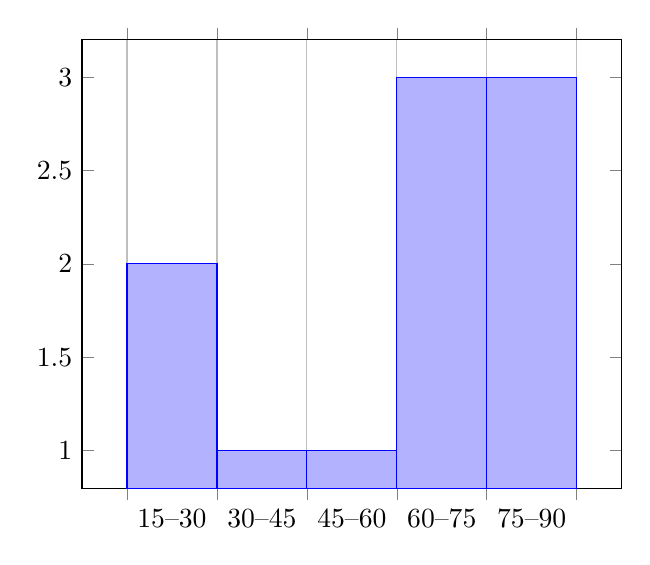
\begin{tikzpicture}
\begin{axis}[
            ybar interval,
            xticklabel=
\pgfmathprintnumber\tick--\pgfmathprintnumber\nexttick
        ]
\addplot+[hist={bins=5}]
            table[row sep=\\,y index=0] {
            data\\
            15\\ 72\\ 55\\ 29\\ 67\\ 89\\ 33\\ 65\\ 78\\ 90\\
            };
\end{axis}
\end{tikzpicture}
\end{figure}

\subsection{Steam and leaf plots}
% http://www.purplemath.com/modules/stemleaf.htm
% TODO describe how its useful to assist in visualizing the shape of a distribution
Steam and leaf plots (The left column of the stem and leaf plot represents the tens place; each number on the right side represents the ones place for the number of pairs of jeans at a department store.)
% TODO draw stem and leaf plot

Next, it must be determined what the stems will represent and what the leaves will represent. Typically, the leaf contains the last digit of the number and the stem contains all of the other digits. In the case of very large numbers, the data values may be rounded to a particular place value (such as the hundreds place) that will be used for the leaves. The remaining digits to the left of the rounded place value are used as the stem.

In this example, the leaf represents the ones place and the stem will represent the rest of the number (tens place and higher).

\section{Standard Data points}
When performing statistical analysis its often helpful to calculate a number of standard data points that helps uncover the nature of the data. Of these the mean, median and mode are all estimates of where the "middle" or "average" of the data is, once these values have been established we can take any observation and see how it relates to the average, for example if we have established that the everage grade is B then a student getting C is below average and a A student is above.

\begin{description}
\item [Mean] Is the sum of the observations divided by the number of observations e.g. the mean of $\{3, 3, 5, 9, 11\}$ is $(3 + 3 + 5 + 9 + 11)/5 = 6.2$. more formally suppose we have a data set containing the values $a_1,\ldots,a_n$, then the arithmetic mean $A$ is defined as
\begin{equation}
A = \frac{1}{n}\sum_{i=1}^{n} a_i
\end{equation}
\item [Median] The "middle" value of the numbers. To find the median arranging all the observations from lowest to highest and pick the middle one (e.g., the median of $\{3, 3, 5, 9, 11\}$ is $5$). If there is an even number of observations then the median is the mean of the two middle values (the median of $\{3, 5, 7, 9\}$ is $(5 + 7) / 2 = 6$).
\item [Mode] The "mode" is the value that occurs most often. If no number is repeated, then there is no mode. e.g. the mode of $\{3, 3, 5, 9, 11\}$ is $3$. In the data set:
$\{1, 1, 1, 2, 2, 2, 3\}$ we see that $1$ and $2$ both have the most occurrences, so they are both modes.
\end{description}

Two less frequently used values are the range and mid-range

\begin{description}
\item [Range] The "range" is the difference between the largest and smallest values. e.g. the range of $\{3, 3, 5, 9, 11\}$ is $11-3=8$.
\item [Mid-range] the mid-range is the arithmetic mean of the maximum and minimum values in a data set
\[
\textrm{MidRange} = \frac{min(x) + max(x)}{2}
\]
\end{description}

% TODO describe their usages
The standard deviation is the average distance between the actual data and the mean.

\subsection{Quartiles}
When using histograms for data analysis we may split the data into any number of groups we deem necessary. This arbitrary split can lead to results that are hard to compare as different researchers may group their data differently. Thus to compare data its useful to group data using a stansafized method, one such method is that of quartiles. With quartiles the data is split into four groups, known as a quartile. Each quartile contains $25\%$ of the total observations. Generally, the data is ordered from smallest to largest with those observations falling below $25\%$ of all the data analysed allocated within the $1st$ quartile, observations falling between $25.1\%$ and $50\%$ and allocated in the $2nd$ quartile, then the observations falling between $51\%$ and $75\%$ allocated in the $3rd$ quartile, and finally the remaining observations allocated in the $4th$ quartile.

When splitting data sets into their quartiles we do so by calculating the boundary values of each quartile known as $Q_1$, $Q_2$ and $Q_3$. Such that

% TODO check this is correct
\begin{itemize}
\item $1st$ quartile $v \in S \text{ where } v < Q_1$
\item $2nd$ quartile $v \in S \text{ where } v > Q_1 \text{ and } v < Q_2$
\item $3rd$ quartile $v \in S \text{ where } v > Q_2 \text{ and } v < Q_3$
\item $4th$ quartile $v \in S \text{ where } v > Q_3$
\end{itemize}

to calculate these we use the following method
\begin{enumerate}\label{stat:quartiles}
    \item Sort data values and find its median, This is $Q_1$.
    \item Divide the data set into two groups: a low group and a high group. When n is odd, the median should be placed in both groups.
    \item Find the median of the low group. This is $Q_1$.
    \item Find the median)of the high group. This is $Q_3$.
\end{enumerate}

Once the quartiles have been determined, its common to calculate the inter-quartile range (IQR)
\begin{equation}
IQR = Q_3 - Q_1
\end{equation}
% TODO why is this useful
A good summary of locations in the distribution is provided by the points that divide the data it into four equally-sized groups. This is the 5-point summary is made of:
\begin{enumerate}
    \item Quartile 0 the minimum
    \item Quartile 1 (bigger than 25\% of the data points)
    \item Quartile 2 (the median)
    \item Quartile 3 (bigger than 75\% of the data points)
    \item Quartile 4 (the maximum)
\end{enumerate}
The five-number summary gives information about the location (from the median), spread (from the quartiles) and range (from the sample minimum and maximum) of the observations
% TODO why is this useful

For example the data set $\{0, 1.5, 2.5, 3, 4, 4, 4, 7, 7.5\}$ has the median $4 = Q_2$. The data to the left of the median is $\{0, 1.5, 2.5, 3\}$ which has $2 = Q_1$ as its median. The data to the right is $\{4, 4, 7, 7.5\}$ which has $5.5 = Q_3$ as its median.

% TODO explain box plots

\begin{tikzpicture}
  \begin{axis}
    \addplot+[
    boxplot prepared={
      median=1,
      upper quartile=1.2,
      lower quartile=0.4,
      upper whisker=1.5,
      lower whisker=0.2
    },
    ] coordinates {};
  \end{axis}
\end{tikzpicture}

\subsection{Distributions}
% TODO http://en.wikipedia.org/wiki/Statistical_dispersion
% TODO draw examples of the different dsitributions
% TODO (symetrical/asymetrical)
% skewed (skewed to the right = right tailed, skewed to the left = left tailex )
% TODO http://stattrek.com/statistics/charts/data-patterns.aspx clusters, gaps, peeks, outliers
% - peek: value where most observations occur
% - gap: a range of values where no observations occur
% - cluster: a group of observatiins sepearetd from other observatiins by gaps
% - outlier: observations seperated by gaps from the main distribution

\subsection{Deviation and variance}
deviation is a measure of difference between the observed value of a variable and some other value, often that variable's mean

% TODO Average absolute deviation http://en.wikipedia.org/wiki/Absolute_deviation#Average_absolute_deviation_.28general_form.29
% TODO mean and median absolute diviation http://en.wikipedia.org/wiki/Median_absolute_deviation
% TODO (Why Square?) http://www.mathsisfun.com/data/standard-deviation.html#WhySquare
% TODO describe usage of and when to use
\begin{description}
    \item [Mean absolute deviation] The mean of the distances of each value from their mean.
\begin{enumerate}
    \item Find the mean of all values
    \item Find the distance of each value from that mean (subtract the mean from each value, ignore minus signs
    \item Then find the mean of those distances
\end{enumerate} For example the Mean Deviation of $3, 6, 6, 7, 8, 11, 15, 16$ is $3.75$ as the mean is $9$ and the distances from this are $6, 3, 3, 2, 1, 2, 6, 7$
\end{description}

The Variance is defined as:

The average of the squared differences from the Mean.

To calculate the variance follow these steps:

Work out the Mean (the simple average of the numbers)
Then for each number: subtract the Mean and square the result (the squared difference).
Then work out the average of those squared differences.

% TODO standard deviation

\section{Regression}
Regression is the main statistical technique used to quantify the relationship between two or more variables. A regression analysis would show a positive relationship between height and weight, for example. The measure of the accuracy of a regression is called R-squared. A perfect relationship, with no error, would have an R-squared of $1.00$ or $100$. Strong relationships, like height and weight, would have an R-squared of around $70$ percent. A meaningless relationship, like hair color and weight, would have an R-squared of zero.

\section{Random samples}
A random sample of $25\%$ of a schools pupules shoved that 16 pupiles had red hair. Based on the data, what is the most reasonable estimate of the total number of pupiles with red hair on the school?. $25\%$ is the same as $1/4$ of the pupiles at the school so the most resonable estimate is $4$ times the number from the sample $4 \cdot 16 = 62$

\section{Exercises}
\begin{ExerciseList}

% TODO MEAN, MEDIAN and MODE excercises

\Exercise Calculate the quartiles of the following data sets
\Question $\{0, 0, 1, 2, 2, 3, 3, 4\}$
\Question $\{3, 4, 4, 5, 5, 5, 6, 7\}$
\Question $\{7, 9, 9, 10, 10, 10, 11, 12, 12, 14\}$
\Question $\{0, 1, 1, 3, 3, 3, 4, 5, 7\}$
\Answer As described in \ref{stat:quartiles} we first calculate $Q_2$ and use its value to find $Q_1$ and $Q_3$
\begin{enumerate}
\item \myindent $Q_2 = 2, Q_1 = 1/2, Q_3 = 3$
\item \myindent $Q_2 = 5, Q_1 = 4, Q_3 = 5.5$
\item \myindent $Q_2 = 10, Q_1 = 9, Q_3 = 12$
\item \myindent $Q_2 = 3, Q_1 = 1, Q_3 = 4.5$
\end{enumerate}

\Exercise Use the normal distrubhtion to answer
\Question normally distributed random variable X has a mean of 20 and a standard deviation of 4. Determine the probability that a randomly selected x-value is between 15 and 22.
\Question The final exam scores in a statistics class were normally distributed with a mean of 58 and a standard deviation of 4. Find the probability that a randomly selected student scored more than 62 on the exam
\Answer TODO

\end{ExerciseList}
